\documentclass[11pt,a4paper]{article}
\usepackage[utf8]{inputenc}
\usepackage[T1]{fontenc}
\usepackage[spanish,es-noquoting]{babel}
\usepackage[margin=2.4cm]{geometry}
\usepackage{booktabs}
\usepackage{enumitem}
\usepackage{parskip}
\usepackage{amsmath}
\usepackage{graphicx}
\usepackage{caption}
\usepackage{abstract}
\graphicspath{{1_documento/Plantilla_de_Tesis___Romina_Carlos/images/}}
\setlist{nosep,leftmargin=1.4em}
\renewcommand{\arraystretch}{1.15}
\captionsetup{font=small,labelfont=bf}
\renewcommand{\abstractnamefont}{\normalfont\bfseries}
\renewcommand{\abstracttextfont}{\normalfont\small}

\title{\vspace{-1.2cm}\bfseries Identificación de familias de ransomware a partir de
artefactos post-ataque: notas de rescate y archivos cifrados como fuentes independientes}
\author{Romina Alfonzo \and Carlos Urdapilleta \\[2pt]
\small Tutor: Prof.\ Cristian Cappo \\[2pt]
\small Facultad Politécnica, Universidad Nacional de Asunción}
\date{\small 12 de agosto de 2026 --- \textit{informe de avance}}

\begin{document}
\maketitle

\begin{abstract}
\noindent Identificar a qué familia pertenece un ataque de ransomware una vez consumado es un
paso previo a cualquier intento de recuperación, porque determina si existe una herramienta de
descifrado conocida. Este trabajo evalúa dos artefactos que la víctima siempre conserva ---la
nota de rescate y los propios archivos cifrados--- como fuentes independientes de
identificación, sin combinarlos, y mide en cada caso qué parte del desempeño corresponde a la
familia y qué parte a la campaña concreta que produjo las muestras. Sobre un corpus de 146
notas de 30 familias, un clasificador supervisado multiclase alcanza un macro-F1 de 0,760
cuando en el entrenamiento aparece la misma plantilla de nota que en la prueba, y de 0,435
cuando se le exige generalizar a una plantilla nunca vista; la separación entre ambos
protocolos se obtiene agrupando las notas por similitud de contenido, procedimiento que revela
que las 146 notas corresponden a solo 95 contenidos distintos. Sobre 14.500 archivos cifrados
de 29 familias del conjunto NapierOne, un clasificador entrenado únicamente sobre los 512
bytes iniciales y los 512 finales de cada archivo ---sin emplear el nombre ni la extensión---
alcanza una exactitud de 0,910, sostenida en 0,879 cuando se evalúa sobre tipos de documento
excluidos del entrenamiento. Ese resultado acota un resultado negativo previo: la
indistinguibilidad de los archivos cifrados es real, pero se limita a seis de las
veintinueve familias evaluadas. Tres intentos independientes de mejora por vía metodológica
---ajuste de hiperparámetros en las notas, abstracción de marcadores variables en las notas y
ajuste de hiperparámetros sobre las características estadísticas de los archivos--- no
produjeron mejora alguna, lo que sitúa el factor limitante en la composición de los datos y no
en el método.

\vspace{4pt}
\noindent\textbf{Palabras clave:} ransomware, identificación de familia, notas de rescate,
archivos cifrados, clasificación multiclase, NapierOne.
\end{abstract}

\section{Introducción}

Cuando un ataque de ransomware ya se ha ejecutado, la pregunta operativa de la víctima no es
si hay una infección sino \emph{de qué familia} se trata. La respuesta condiciona todo lo
demás: si existe una herramienta pública de descifrado, si la clave se filtró alguna vez, si
el grupo responsable acostumbra a exfiltrar datos además de cifrarlos. El binario que ejecutó
el cifrado suele haberse eliminado a sí mismo, y el tráfico de red asociado ya ocurrió. Lo
que queda, invariablemente, son dos artefactos: la nota de rescate y los archivos cifrados.

Este trabajo estudia ambos como fuentes de identificación de familia, y lo hace
deliberadamente por separado. No se propone un sistema que los combine. La razón es que cada
uno tiene una naturaleza distinta ---uno es texto redactado por personas, el otro es la salida
de un programa--- y mezclarlos antes de saber cuánto aporta cada uno impediría atribuir el
resultado. La decisión resultó además informativa: como se verá en la Sección \ref{sec:disc},
las familias que el análisis de archivos no resuelve son precisamente aquellas para las que la
nota es la única vía disponible.

La contribución que este informe reporta es de tres tipos. Primero, una medición separada de
dos escenarios de evaluación que la literatura suele confundir: reconocer una familia cuya
plantilla de nota ya se conoce, y reconocerla a partir de una variante nunca vista. Segundo,
la demostración de que la familia de un archivo cifrado es identificable a partir de su
contenido, sin recurrir al nombre ni a la extensión, con una exactitud de 0,910 sobre 29
familias. Tercero, tres resultados negativos convergentes que delimitan dónde está el techo
actual del problema.

\section{Trabajos relacionados}

El antecedente directo es Lemmou, Lanet y Souidi \cite{lemmou2021}, que analizan en
profundidad los archivos de nota de rescate y \emph{sí} identifican la familia a partir de
ellos. Conviene precisar su método, porque de él se desprende con exactitud qué queda por
hacer. Su identificador de familia es un prototipo basado en reglas y marcadores: extrae
correos electrónicos, direcciones Bitcoin y Bitmessage, direcciones \texttt{.onion}, nombres
de familia y palabras clave, y emplea análisis semántico latente como búsqueda de
casi-duplicados con un umbral de 0,99995 contra su propia base de 176 notas de 62 familias.
Con ello identifica 181 de 182 notas. Es un escenario de mundo cerrado, sin partición entre
entrenamiento y prueba. Su componente de aprendizaje automático, en cambio, resuelve una tarea
distinta y binaria ---decidir si un nombre de archivo corresponde a una nota de rescate o a un
archivo benigno--- con F de 0,920 y exactitud de 98,32\,\%.

Lo que ese trabajo no aborda, y este sí, es un clasificador supervisado multiclase sobre el
contenido completo de la nota, con medición explícita de la generalización a variantes no
vistas y con métricas macro. Las dos aproximaciones son complementarias: un identificador por
marcadores requiere una base curada de indicadores que envejece con cada campaña nueva,
mientras que un clasificador entrenado sobre contenido no la necesita, pero paga el precio de
depender de la diversidad del corpus de entrenamiento.

Trujillo \cite{trujillo2022} aborda la detección binaria de notas por contenido con árboles de
decisión y máquinas de vectores de soporte sobre 59 notas y 59 documentos benignos, y aporta un
elemento metodológico de interés: una validación temporal, entrenando con notas anteriores a
julio de 2019 y evaluando sobre notas posteriores.

En el frente de los archivos cifrados, Pont y Hernández-Castro \cite{pont2020} argumentan por
qué los enfoques estadísticos de detección de ransomware fallan, un resultado que este trabajo
matiza más que contradice: la entropía global efectivamente no discrimina, pero las
estadísticas regionales sí lo hacen en grado apreciable. Davies, Macfarlane y Buchanan
publicaron el conjunto de datos NapierOne \cite{napierone2021}, empleado aquí, y más tarde un
esquema de detección por votación mayoritaria \cite{davies2023} en el que proponen
explícitamente, como línea futura, aplicar procesamiento de lenguaje natural sobre las cadenas
de texto de las notas: es el hueco que este trabajo aborda, señalado por el propio grupo
creador del conjunto de datos.

\section{Materiales y métodos}

\subsection{Corpus de notas de rescate}

El corpus consta de 146 notas correspondientes a 30 familias, reunidas a partir de
repositorios públicos ---ThreatLabz/Zscaler, el repositorio asociado a
Lemmou et al.\ \cite{lemmou2021} y portales de análisis de seguridad. La procedencia de 37 de
las notas quedó registrada de forma ambigua en el manifiesto y está pendiente de auditoría;
se declara aquí como limitación de trazabilidad.

Las notas llegan en texto plano, HTML, RTF y HTA. La extracción exigió detectar la
codificación de cada archivo mediante marca de orden de bytes y, en su ausencia, mediante la
proporción de bytes nulos, con retroceso a \texttt{cp1252}: sin ese tratamiento, 13 notas de
tres familias entraban al vectorizador como vectores vacíos, y sus bytes nulos actuaban como
firma sintética de familia.

\subsection{Los dos protocolos de evaluación}
\label{sec:protocolos}

El hallazgo que determina el diseño experimental es que las notas de rescate son
\textbf{plantillas}. Agrupando las 146 notas por similitud del coseno superior a 0,90 sobre
n-gramas de caracteres, resultan solo \textbf{95 contenidos distintos}: DHARMA aporta 19 notas
que corresponden a 6 plantillas, y WASTEDLOCKER aporta 4 notas que son una sola.

Evaluar sin tener en cuenta esa estructura mezcla dos preguntas distintas. De ahí que todo
resultado se reporte bajo dos protocolos:

\begin{itemize}
\item \textbf{P1, «plantilla conocida»}: validación cruzada estratificada. En el entrenamiento
pueden aparecer otras notas de la misma plantilla que la nota de prueba. Responde a: dada una
familia cuyo repertorio de notas ya se conoce, ¿se la reconoce? Es el escenario comparable con
las herramientas de identificación existentes.
\item \textbf{P2, «variante nunca vista»}: validación cruzada estratificada \emph{por grupos},
donde el grupo es la plantilla. Ninguna nota de la plantilla de prueba aparece en el
entrenamiento. Responde a: ¿se reconoce la familia ante una campaña nueva?
\end{itemize}

Ambos protocolos se ejecutan con 2 particiones y 10 semillas, y se reporta la media con su
desvío. La vectorización TF-IDF se realiza dentro de un \emph{pipeline}, de modo que el
vocabulario y los pesos IDF se ajustan solo sobre la partición de entrenamiento; hacerlo
fuera filtra información de la prueba. Se emplean tres representaciones ---n-gramas de
palabras (1--2), n-gramas de caracteres con frontera de palabra (3--5) y su combinación--- y
cuatro modelos: LinearSVC, regresión logística, Random Forest y $k$ vecinos más próximos.

\subsection{Corpus de archivos cifrados}

Se emplea el conjunto NapierOne \cite{napierone2021}, en el que un mismo conjunto base de
documentos fue cifrado por muestras reales de distintas familias, lo que permite comparar el
efecto de cada una sobre contenidos idénticos. Los experimentos usan 29 familias, con tamaños
de muestra distintos según el costo de cada uno: 29.029 archivos (1.001 por familia) para las
características estadísticas, 1.450 (50 por familia) para el análisis estructural y 14.500
(500 por familia) para el clasificador final.

\subsection{Métricas}

Se reporta exactitud, exactitud balanceada y \textbf{macro-F1}, esta última como métrica
principal. La razón es que el corpus está desbalanceado, y una métrica ponderada queda
dominada por las familias mejor representadas: promediar el F1 de las familias por igual
impide que un buen desempeño sobre DHARMA compense el fracaso sobre una familia con dos notas.
El azar corresponde a 0,033 en el frente de notas (30 familias) y a 0,034 en el de archivos
(29 familias).

\subsection{Infraestructura}

Los experimentos que exceden la capacidad de un equipo personal se ejecutaron en el clúster
computacional del NIDTEC (FP-UNA) mediante SLURM. La corrección de tres fallas de
paralelismo anidado y de asignación de memoria forma parte del registro metodológico del
trabajo.

\section{Resultados}

\subsection{Frente de notas de rescate}

\begin{table}[h]
\centering\small
\caption{Identificación de familia a partir de la nota de rescate. 146 notas, 30 familias,
95 plantillas. Media de 10 semillas.}
\begin{tabular}{@{}llccc@{}}
\toprule
\textbf{Protocolo} & \textbf{Mejor configuración} & \textbf{Exactitud} & \textbf{Exac.\ bal.} & \textbf{Macro-F1} \\
\midrule
P1 --- plantilla conocida & caracteres + LinearSVC & 0,818 & 0,777 & $\mathbf{0{,}760 \pm 0{,}029}$ \\
P2 --- variante nunca vista & combinado + LinearSVC & 0,551 & 0,492 & $\mathbf{0{,}435 \pm 0{,}057}$ \\
\midrule
\multicolumn{2}{@{}l}{Azar (30 familias)} & \multicolumn{3}{c}{0,033} \\
\bottomrule
\end{tabular}
\end{table}

La brecha entre ambos protocolos ---0,325 puntos de macro-F1--- es el resultado principal de
este frente, y admite una lectura precisa: haber visto una plantilla de una familia ayuda poco
a reconocer otra plantilla de la misma familia. No obstante, 0,435 está trece veces por encima
del azar, de modo que las plantillas de una misma familia comparten \emph{algo}; ese resto
compartido, todavía no caracterizado, es el objeto natural del trabajo siguiente.

En el escenario P1, que es el comparable con las herramientas de identificación por nota
disponibles, la exactitud de 0,818 supera el 71,93\,\% obtenido al evaluar una herramienta
pública de identificación en un experimento propio de este trabajo.

\subsubsection*{Dos intentos de mejora sin efecto}

Se ensayaron dos vías de mejora sobre este frente, ambas sin resultado.

La primera fue una \textbf{búsqueda anidada de hiperparámetros} ---840 configuraciones, con la
búsqueda contenida dentro de la partición de entrenamiento para no contaminar la evaluación---
que arrojó P1 $= 0{,}775 \pm 0{,}032$ y P2 $= 0{,}424 \pm 0{,}064$, frente a 0,783 y 0,427 sin
ajuste alguno sobre la misma base. Las diferencias caen dentro del desvío entre semillas.

La segunda fue la \textbf{abstracción de los marcadores variables}: sustituir correos,
direcciones \texttt{.onion}, direcciones Bitcoin, URLs e identificadores de víctima por
etiquetas de tipo, con la hipótesis de que el modelo memorizaba valores concretos que cambian
entre campañas y que aprender el patrón sería más estable. Se modificaron 130 de 144 notas con
1.281 sustituciones. El efecto fue de $-0{,}010$ en P2 y $-0{,}005$ en P1: nulo, y la
representación de caracteres fue la que más perdió, lo que sugiere que los n-gramas extraían
señal de la \emph{forma} de los marcadores ---la longitud de una dirección \texttt{.onion}, el
formato de una URL--- y que la etiqueta uniforme la destruye.

La conclusión conjunta es que la variabilidad entre plantillas de una misma familia es
\textbf{estructural} y no se reduce a los datos de contacto.

\subsection{Frente de archivos cifrados}

\subsubsection{Las propiedades estadísticas: el resultado negativo, acotado}

El punto de partida de este frente era un resultado negativo: la entropía del archivo cifrado
no permite distinguir familias. Ampliando el espacio de características a 275 y evaluando
sobre 29.029 archivos, ese enunciado resulta cierto solo en su versión estricta.

\begin{table}[h]
\centering\small
\caption{Identificación de familia por características estadísticas. 29.029 archivos, 29
familias. Macro-F1.}
\begin{tabular}{@{}lccc@{}}
\toprule
\textbf{Conjunto de características} & \textbf{Random Forest} & \textbf{KNN-5} & \textbf{HistGB} \\
\midrule
Entropía global $+$ tamaño (2) & 0,166 & 0,126 & 0,163 \\
Estadísticas globales (9) & 0,391 & 0,300 & 0,399 \\
Frecuencia de bytes (256) & 0,184 & 0,082 & 0,199 \\
Todas (275) & 0,542 & 0,143 & 0,592 \\
\textbf{Estadísticas $+$ derivadas (19)} & $\mathbf{0{,}603}$ & 0,299 & 0,598 \\
\bottomrule
\end{tabular}
\end{table}

Dos observaciones. La primera es que el resultado depende de \emph{qué} se mide, no de cuánto:
la entropía global del archivo completo casi no discrimina (0,166), mientras que las
estadísticas regionales y de rachas alcanzan 0,603. La segunda es que 275 características
rinden peor que 19 bien elegidas ---0,592 frente a 0,603---: las 256 frecuencias de byte
agregan ruido. Una selección automática por ANOVA obtuvo entre 0,363 y 0,387, por debajo de
las 19 elegidas manualmente.

El motivo de que las estadísticas regionales funcionen queda a la vista en las importancias
del Random Forest, que son estructurales y no criptográficas: la racha más larga de bytes
repetidos (0,072), la diferencia de entropía entre cabecera y cola (0,041), la entropía de la
cola (0,040) y la de la cabecera (0,031). Todas miden la presencia de datos \emph{no}
aleatorios añadidos al archivo.

Una búsqueda de hiperparámetros sobre este experimento ---cuatro configuraciones, hasta 2,5
horas de cómputo cada una--- devolvió valores entre 0,599 y 0,603. La diferencia respecto del
valor sin ajustar es de $-0{,}000$.

\subsubsection{Los artefactos estructurales}

Si lo que discrimina es la presencia de datos no aleatorios, cabe buscarlos directamente. Un
procedimiento que descubre automáticamente, sin catálogo previo, el prefijo y el sufijo
binario común a los archivos de cada familia, halló marca en \textbf{25 de 29 familias} sobre
1.450 archivos. Varias de esas marcas son legibles como texto, porque son cadenas que el
propio programa escribe para reconocer lo que ya cifró: WANNACRY inserta
\texttt{57~41~4E~41~43~52~59~21} (\guillemotleft WANACRY!\guillemotright), CUBA un prefijo de
20 bytes que se lee \guillemotleft FIDEL.CA\guillemotright{} y PHOBOS uno de 7 con
\guillemotleft LOCK96\guillemotright. CERBER, LOCKBIT, RANSOMEXX y TESLACRYPT presentan firmas
de 64 bytes. Once de las quince firmas están al final del archivo y solo cuatro al principio.

La ablación de este experimento es la parte que más importa, y obliga a no reportar su
resultado global:

\begin{table}[h]
\centering\small
\caption{Ablación del análisis estructural. 1.450 archivos, 29 familias.}
\begin{tabular}{@{}lccc@{}}
\toprule
\textbf{Modo} & \textbf{Cobertura} & \textbf{Exactitud global} & \textbf{Exactitud donde aplica} \\
\midrule
Solo extensión del archivo & 82,8\,\% & 82,8\,\% & \textbf{100\,\%} \\
Solo firmas binarias & 53,3\,\% & 51,7\,\% & \textbf{97,0\,\%} \\
Combinado & 87,8\,\% & 86,2\,\% & 98,2\,\% \\
\bottomrule
\end{tabular}
\end{table}

La extensión explica casi todo el resultado global y acierta el 100\,\% cuando está presente,
pero eso no es identificación de familia: es identificación de \textbf{campaña}. Una campaña es
un despliegue concreto de una familia, con una compilación, una configuración de contacto y una
extensión propias; la misma familia lanza campañas sucesivas y cambia esos datos en cada una.
En NapierOne cada familia fue cifrada ejecutando una única muestra una única vez, de modo que
todos sus archivos comparten extensión. Un clasificador que la use no aprende la familia,
aprende esa campaña, y no sobreviviría a un cambio de extensión. Las firmas binarias, en
cambio, son el hallazgo defendible: cubren la mitad del corpus, pero allí identifican al
97\,\%, y al residir en el contenido son más estables entre campañas.

Cuatro familias no dejan marca alguna: BADRABBIT, JIGSAW, NOTPETYA y SUNCRYPT. El caso de
NOTPETYA coincide con lo documentado por Davies et al.\ \cite{davies2023} por una vía
metodológica distinta.

\subsubsection{Aprendizaje sobre los bytes del archivo}

La regla de coincidencia exacta cubre solo el 53\,\% de los archivos. Para el resto se
entrenó un clasificador sobre una representación posicional de los \textbf{512 primeros y 512
últimos bytes} de cada archivo, \textbf{sin utilizar el nombre ni la extensión}.

\begin{table}[h]
\centering\small
\caption{Clasificación de familia sobre el contenido del archivo. Sin metadatos.}
\begin{tabular}{@{}lccc@{}}
\toprule
\textbf{Configuración} & \textbf{$n$} & \textbf{Exactitud} & \textbf{Macro-F1} \\
\midrule
Posicional $+$ Random Forest (búsqueda anidada) & 5.800 & 0,897 & 0,897 \\
n-gramas de bytes $+$ regresión logística & 5.800 & 0,856 & 0,858 \\
n-gramas de bytes $+$ LinearSVC & 5.800 & 0,849 & 0,846 \\
\textbf{Final: posicional $+$ Random Forest} & \textbf{14.500} & $\mathbf{0{,}910}$ & $\mathbf{0{,}908}$ \\
\bottomrule
\end{tabular}
\end{table}

Que la representación posicional supere a los n-gramas indica que las marcas residen en
\emph{desplazamientos fijos} y no dispersas por el archivo. Es un dato metodológico que
contrasta con el frente de notas, donde los n-gramas de caracteres son los que mejor funcionan.

El desempeño es marcadamente bimodal. \textbf{Veintitrés de las veintinueve familias obtienen
F1 $\geq 0{,}98$}. Las seis restantes son SUNCRYPT (0,75), WASTEDLOCKER (0,64), CRYPTOLOCKER
(0,61), DARKSIDE (0,60), JIGSAW (0,44) y NOTPETYA (0,38), y forman un grupo de confusión
mutua: entre el 97,2\,\% y el 99,4\,\% de sus errores caen dentro del propio grupo. DARKSIDE
actúa como sumidero, con precisión de 0,45 y exhaustividad de 0,90: absorbe los archivos
ambiguos de las demás.

La correspondencia con el experimento estructural funciona como validación cruzada entre
experimentos. Las quince familias con firma binaria obtienen aquí F1 $\geq 0{,}99$ sin
excepción. De las diez que solo tenían extensión, siete llegan igualmente a 0,99, lo que
significa que el aprendizaje encuentra patrones de contenido que la regla exacta no detecta. Y
de las cuatro sin marca alguna, BADRABBIT pasa de 0,15 a 0,98.

\subsection{Validación y localización de la señal}

\subsubsection*{¿Aprende del ransomware o del documento original?}

En NapierOne todas las familias cifraron el mismo conjunto base de documentos, por lo que cabía
la sospecha de que el clasificador aprendiera rasgos del documento de origen. La validación
\emph{dejar-un-tipo-fuera} ---entrenar con todos los tipos de documento salvo uno y evaluar
sobre ese--- lo descarta: promediando siete tipos, la exactitud es de 0,879 y el macro-F1 de
0,861, frente a 0,910 con el tipo presente en el entrenamiento. La caída es de $-0{,}031$. El
peor caso es \texttt{jpg} (0,874), cuya estructura interna nada tiene que ver con la de un
documento de oficina. Las familias que sustituyen el nombre original por cadenas aleatorias
---BLACKMATTER y CERBER, 491 archivos--- participan del entrenamiento pero no de la prueba;
CERBER obtiene F1 de 1,00 pese a que ningún método basado en el nombre podría identificarla.

\subsubsection*{¿Dónde está la información?}

La importancia acumulada del modelo se reparte en 0,204 para la cabecera y \textbf{0,796 para
la cola}: el ransomware firma al final del archivo. Los desplazamientos más informativos son
$-5$, $-133$, $-1$, $-2$, $-3$ y $-6$ respecto del final. Converge con el análisis estructural,
donde once de las quince firmas son sufijos, y tiene una explicación mecánica: añadir un bloque
de control al final es más simple que insertarlo al principio, lo que obligaría a desplazar
todo el contenido.

\begin{table}[h]
\centering\small
\caption{Ablación de la ventana de lectura. Exactitud.}
\begin{tabular}{@{}lcc@{}}
\toprule
\textbf{Ventana} & \textbf{Bytes leídos} & \textbf{Exactitud} \\
\midrule
64 $+$ 64 & 128 & 0,795 \\
128 $+$ 128 & 256 & 0,793 \\
256 $+$ 256 & 512 & 0,852 \\
512 $+$ 512 & 1.024 & \textbf{0,908} \\
Solo cabecera & 512 & 0,321 \\
Solo cola & 512 & 0,752 \\
\bottomrule
\end{tabular}
\end{table}

Con 128 bytes se alcanza el 87\,\% del rendimiento máximo, dato relevante para una
implementación práctica. La cola por sí sola más que duplica a la cabecera por sí sola, pero
ambas regiones son necesarias para el máximo: su combinación suma quince puntos sobre la cola
aislada.

\subsubsection*{Por qué fallan las seis familias difíciles}

No fallan todas por el mismo motivo, y la distinción importa.

\begin{table}[h]
\centering\small
\caption{Entropía media de cabecera y cola en las seis familias de bajo desempeño.}
\begin{tabular}{@{}lcc@{}}
\toprule
\textbf{Familia} & \textbf{Entropía cabecera} & \textbf{Entropía cola} \\
\midrule
CRYPTOLOCKER & 7,59 & 7,59 \\
WASTEDLOCKER & 7,59 & 7,58 \\
JIGSAW & 7,51 & 7,55 \\
DARKSIDE & 7,59 & 7,49 \\
\textbf{SUNCRYPT} & 7,59 & \textbf{4,78} \\
\textbf{NOTPETYA} & 7,34 & \textbf{6,58} \\
\midrule
Resto de familias & 7,03 & 7,44 \\
\bottomrule
\end{tabular}
\end{table}

Las cuatro primeras presentan entropía próxima al máximo en todo el archivo: el cifrado lo
ocupa por completo y no hay marca que aprender. SUNCRYPT y NOTPETYA, en cambio, \emph{sí}
añaden datos no aleatorios al final ---SUNCRYPT tiene la entropía de cola más baja de todo el
conjunto--- y aun así no se identifican. La explicación más plausible es que ese bloque varía
en cada archivo, por tratarse de una clave o de un identificador por víctima: constituye
estructura, pero no firma de familia. La verificación directa de esta hipótesis, mediante
comparación hexadecimal de la cola entre varias muestras, está pendiente y hasta entonces se
formula como conjetura.

\subsection{Síntesis del frente de archivos}

\begin{table}[h]
\centering\small
\caption{Progresión del frente de archivos cifrados. La cobertura indica qué fracción de los
archivos el método es capaz de clasificar.}
\begin{tabular}{@{}lccc@{}}
\toprule
\textbf{Enfoque} & \textbf{Exactitud} & \textbf{Cobertura} & \textbf{Usa metadatos} \\
\midrule
Entropía global $+$ tamaño & 0,166 & 100\,\% & no \\
19 estadísticas regionales & 0,603 & 100\,\% & no \\
Firmas binarias exactas & 0,517 \small(0,97 donde aplica) & 53\,\% & no \\
Extensión del archivo & 0,828 & 83\,\% & \textbf{sí (campaña)} \\
\textbf{Aprendizaje sobre bytes} & $\mathbf{0{,}910}$ & \textbf{100\,\%} & \textbf{no} \\
\bottomrule
\end{tabular}
\end{table}

\begin{figure}[h]
\centering
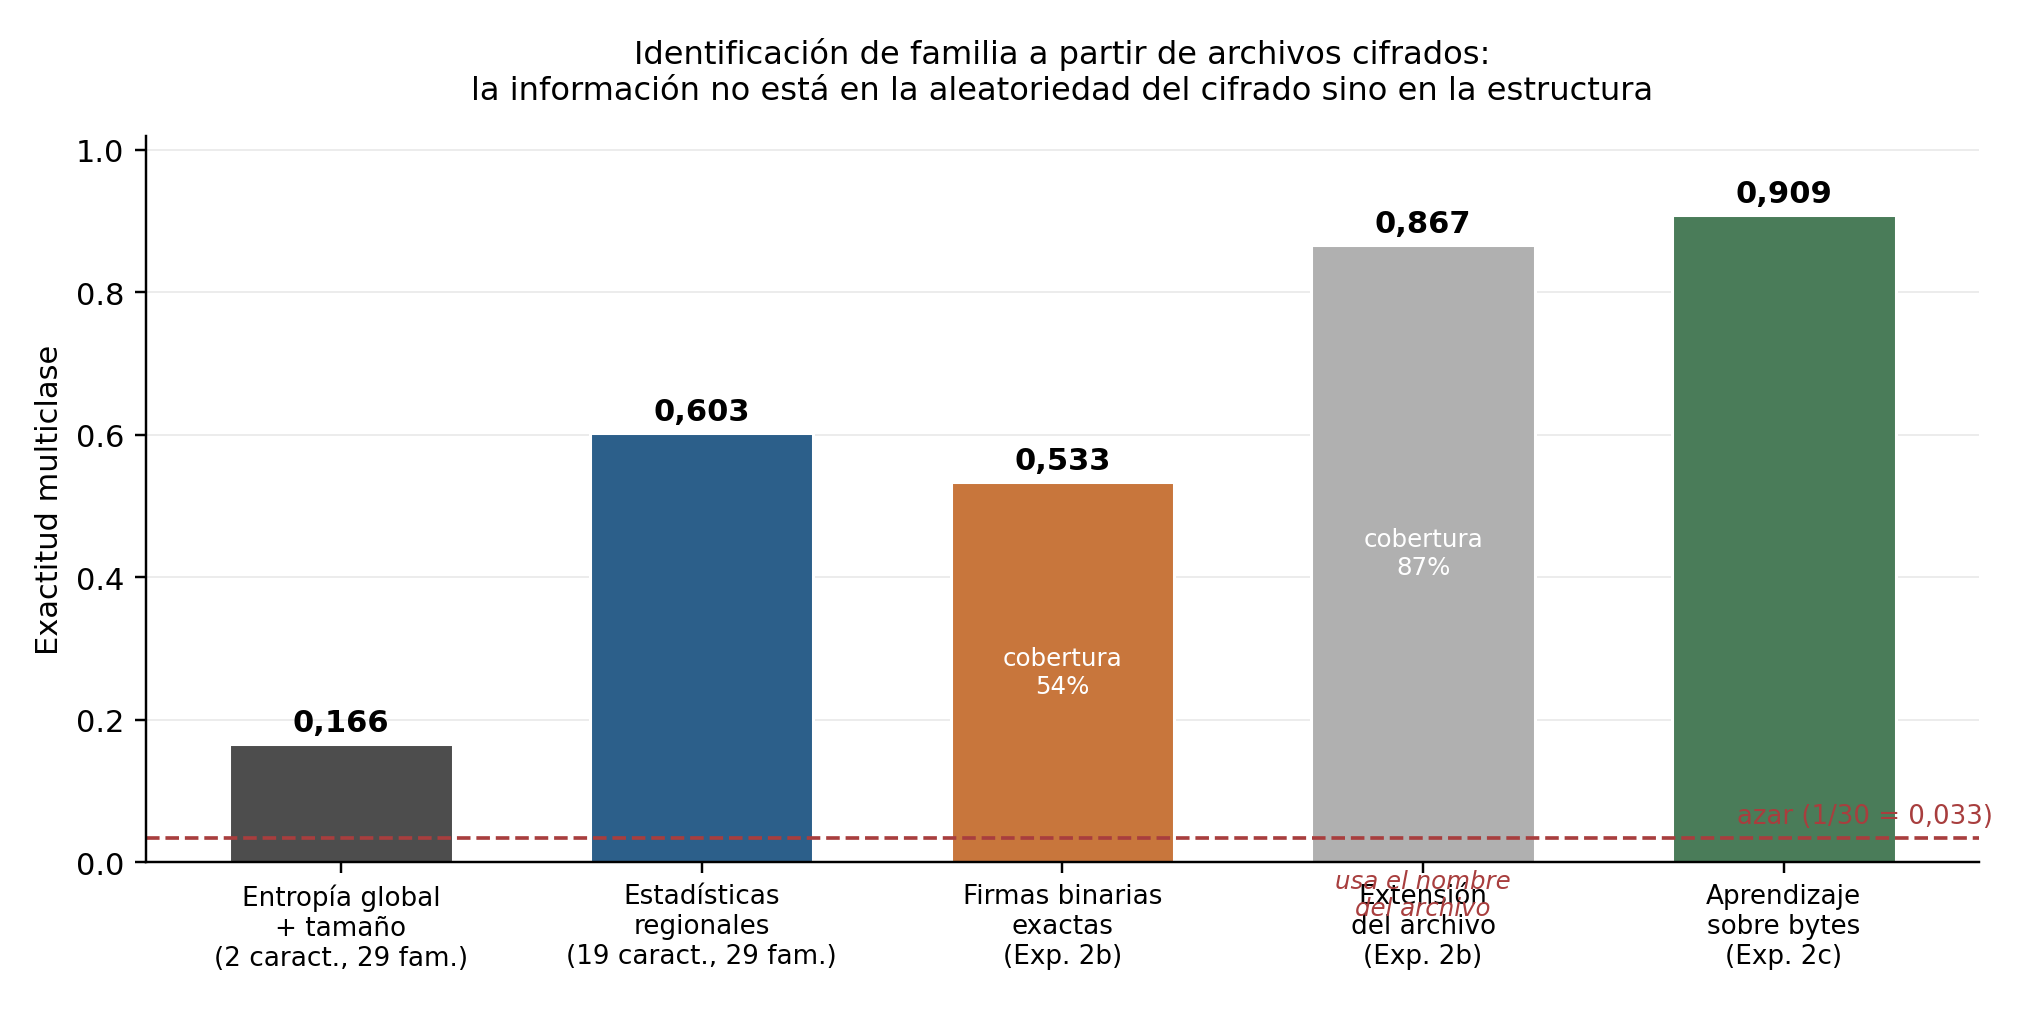
\includegraphics[width=0.78\textwidth]{fig_progresion_archivos.png}
\caption{Progresión del desempeño en el frente de archivos cifrados. Cada etapa responde a una
objeción de la anterior. La barra de la extensión se distingue porque identifica la campaña
concreta y no la familia.}
\end{figure}

El resultado negativo de partida queda así \textbf{acotado a seis de las veintinueve
familias}: la indistinguibilidad estadística es real, pero solo para aquellas que cifran sin
dejar estructura. Para las otras veintitrés la información está en el contenido y es
extraíble.

\section{Discusión}
\label{sec:disc}

\subsection{Una misma lección desde dos artefactos distintos}

Los dos frentes, estudiados por separado y con metodologías que no comparten nada ---uno
procesa texto redactado por personas, el otro la salida binaria de un programa---, arrojan la
misma estructura de resultado. En ambos coexisten dos señales que conviene no confundir: una
fácil de explotar pero ligada a la campaña concreta, y otra más difícil pero propia del
contenido.

\begin{table}[h]
\centering\small
\caption{Simetría entre los dos frentes.}
\begin{tabular}{@{}lll@{}}
\toprule
\textbf{Frente} & \textbf{Señal ligada a la campaña} & \textbf{Señal de contenido} \\
\midrule
Notas de rescate & plantilla conocida: 0,760 & variante nueva: 0,435 \\
Archivos cifrados & extensión: 0,828 & bytes del archivo: 0,910 \\
\bottomrule
\end{tabular}
\end{table}

\begin{figure}[h]
\centering
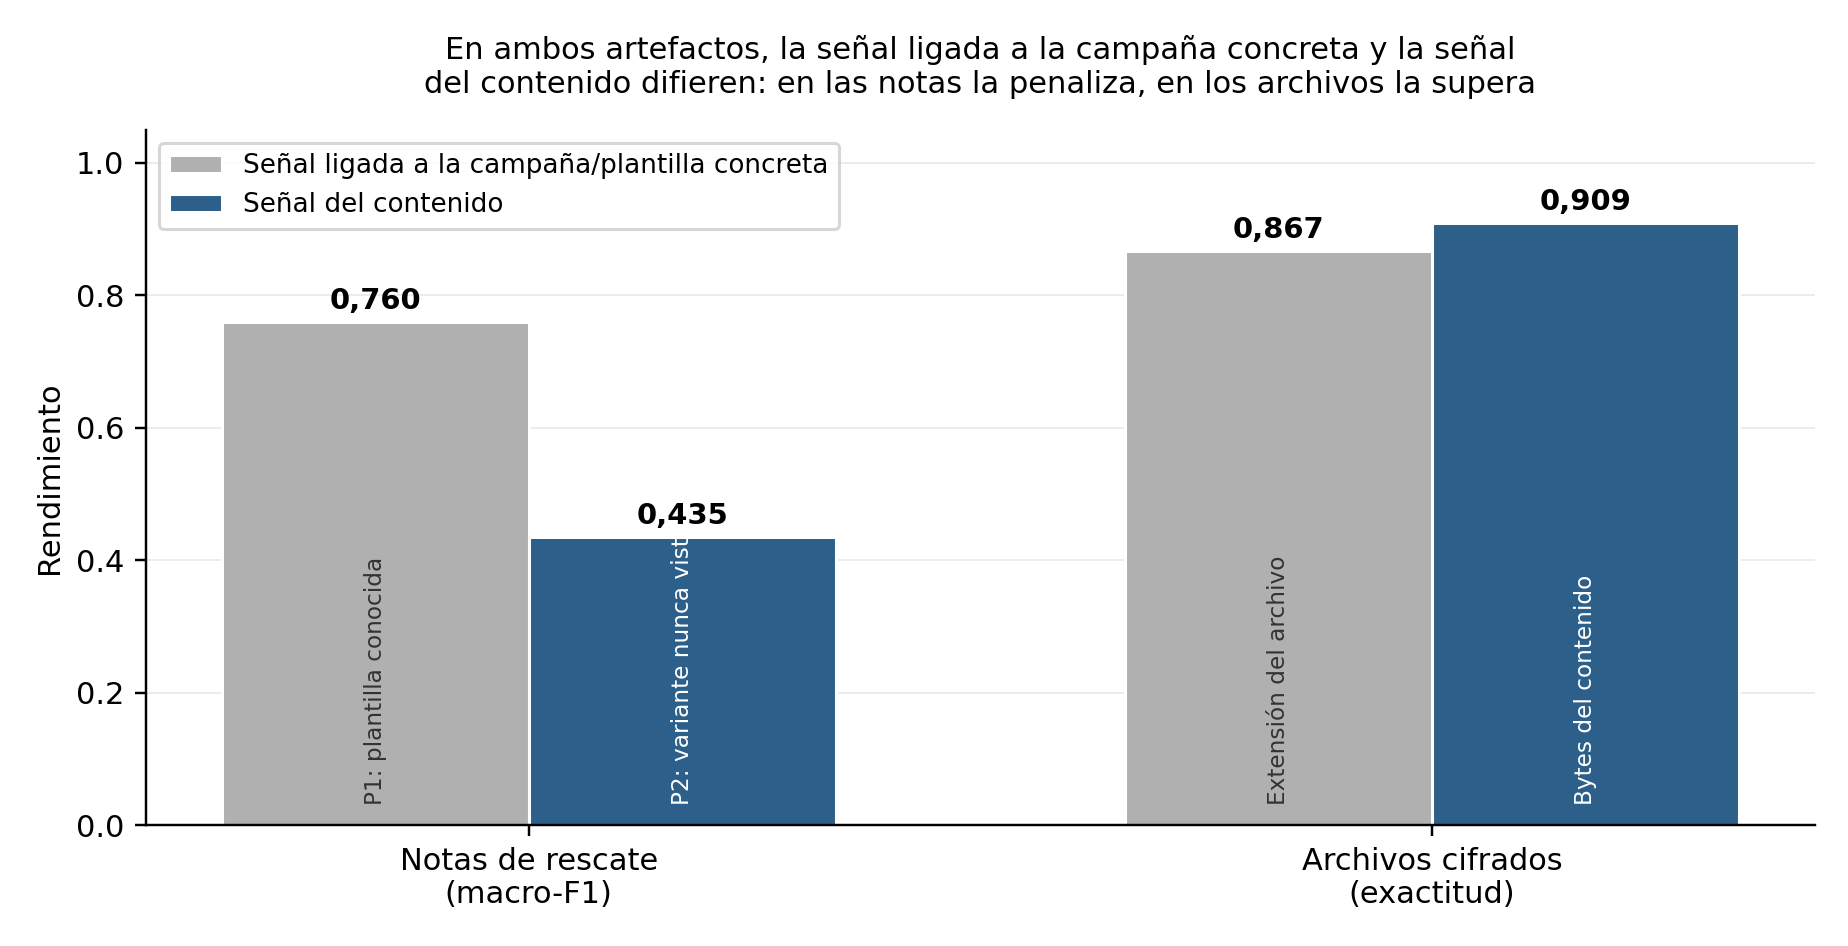
\includegraphics[width=0.72\textwidth]{fig_simetria_frentes.png}
\caption{Señal ligada a la campaña frente a señal de contenido, en los dos artefactos.}
\end{figure}

La lectura conjunta explica por qué las herramientas basadas en catálogos de reglas funcionan
bien sobre campañas conocidas y requieren actualización permanente: operan sobre la señal
fácil. Y señala dónde debe medirse el progreso real: en la señal de contenido, que en el frente
de archivos ya supera a la de campaña (0,910 frente a 0,828) y en el de notas todavía no
(0,435 frente a 0,760).

\subsection{Las seis familias difíciles justifican mantener los frentes separados}

Las seis familias que el análisis de archivos no resuelve son precisamente los casos en que la
nota de rescate constituye la única vía de identificación disponible. La decisión de no
combinar los artefactos, tomada al inicio por razones de atribución de resultados, queda así
respaldada por los datos: no se trata de dos métodos redundantes cuya fusión mejoraría un
promedio, sino de dos métodos cuyas zonas de fallo no coinciden.

\subsection{Tres resultados negativos convergentes}

Tres intentos independientes de mejora por vía metodológica no produjeron efecto: el ajuste de
hiperparámetros del clasificador de notas (840 configuraciones), la abstracción de marcadores
variables en las notas (130 notas modificadas, 1.281 sustituciones) y el ajuste de
hiperparámetros sobre las características estadísticas de los archivos (cuatro
configuraciones). Los tres apuntan a la misma conclusión: \textbf{el techo actual no está en el
método sino en los datos}. En las notas, en la cantidad de plantillas disponibles por familia;
en los archivos, en la cantidad de campañas por familia, que es una sola.

Reportarlos tiene valor propio: cierra la objeción de si se intentó optimizar los modelos, y
redirige el esfuerzo restante hacia donde puede rendir.

\section{Limitaciones}

\begin{itemize}
\item \textbf{Una campaña por familia.} NapierOne representa cada familia mediante una única
ejecución de una única muestra. La exactitud de 0,910 mide identificación de esa campaña; la
generalización a campañas nuevas de la misma familia \emph{no es evaluable} con este conjunto
de datos. Es el análogo exacto de las plantillas en el frente de notas, y la limitación más
importante del trabajo. Ampliar la descarga a una escala mayor del mismo conjunto no la
resuelve, porque añadiría más archivos de la misma campaña.
\item \textbf{Diversidad de plantillas en las notas.} Siete familias están representadas por
una única plantilla y por tanto son inevaluables bajo P2. Las fuentes públicas ya fueron
recolectadas de forma sistemática, de modo que la ampliación depende de la disponibilidad de
terceros y no del esfuerzo propio.
\item \textbf{Trazabilidad del corpus de notas.} La procedencia de 37 de las 146 notas está
pendiente de auditoría.
\item \textbf{Integridad del corpus.} Dos notas del corpus fueron puestas en cuarentena por el
antivirus del equipo de trabajo, por tratarse de archivos HTA reales. Las cifras canónicas del
frente de notas corresponden a 146 notas y las de los dos experimentos de mejora a 144; ambos
valores se declaran por separado y no se mezclan.
\item \textbf{Alcance del enunciado sobre las familias difíciles.} No es correcto afirmar que
las seis familias de bajo desempeño no dejan estructura: dos de ellas sí lo hacen. La
naturaleza de ese bloque final permanece sin verificar.
\end{itemize}

\section{Conclusiones preliminares y trabajo en curso}

Este informe reporta el estado de un trabajo en desarrollo y sus conclusiones son, por tanto,
provisionales.

La familia de ransomware es identificable a partir de un archivo cifrado leyendo únicamente
1.024 bytes de su contenido, sin recurrir al nombre ni a la extensión, con una exactitud de
0,910 sobre 29 familias que se sostiene en 0,879 frente a tipos de documento nunca vistos.
El resultado negativo del que partía este frente ---la indistinguibilidad estadística de los
archivos cifrados--- es cierto, pero acotado a seis familias, y de ellas dos fallan por una
razón distinta de la que se les suponía.

A partir de la nota de rescate, la identificación alcanza un macro-F1 de 0,760 cuando la
plantilla es conocida y de 0,435 cuando no lo es. La distancia entre ambas cifras, y no
ninguna de las dos por separado, es la medida honesta del estado del problema: las
herramientas existentes operan en el primer escenario, y el segundo es el que corresponde a un
ataque con una campaña nueva.

El trabajo en curso se dirige a tres frentes. Primero, documentar con precisión el límite que
impone la composición del corpus, reportando el desempeño estratificado según la cantidad de
plantillas disponibles por familia, lo que establece cuántas plantillas son necesarias para que
la generalización sea posible. Segundo, evaluar enfoques de aprendizaje con pocos ejemplos para
las familias representadas por una o dos plantillas, única vía metodológica cuando la
recolección no puede aportar más muestras. Tercero, verificar la naturaleza del bloque final en
SUNCRYPT y NOTPETYA, para convertir en hecho lo que hoy es conjetura.

\subsection*{Agradecimientos}

Los experimentos de mayor costo computacional se ejecutaron en el clúster del Núcleo de
Investigación y Desarrollo Tecnológico (NIDTEC) de la Facultad Politécnica, Universidad
Nacional de Asunción.

\begin{thebibliography}{9}
\small

\bibitem{lemmou2021}
Lemmou, Y., Lanet, J.-L. y Souidi, E.M. (2021).
\textit{In-Depth Analysis of Ransom Note Files}.
Computers, 10(11):145.

\bibitem{napierone2021}
Davies, S.R., Macfarlane, R. y Buchanan, W.J. (2021).
\textit{NapierOne: A Modern Mixed File Data Set Alternative to Govdocs1}.
Forensic Science International: Digital Investigation.

\bibitem{davies2023}
Davies, S.R., Macfarlane, R. y Buchanan, W.J. (2023).
\textit{Majority Voting Approach to Ransomware Detection}.
arXiv:2305.18852.

\bibitem{pont2020}
Pont, J. y Hernández-Castro, J. (2020).
\textit{Why Current Statistical Approaches to Ransomware Detection Fail}.
23rd Information Security Conference (ISC), pp.\ 199--218.

\bibitem{trujillo2022}
Trujillo, K.K. (2022).
\textit{Ransomware note detection techniques using supervised machine learning}.
Tesis de máster, Universitat Politècnica de Catalunya.

\end{thebibliography}

\end{document}
